%============================================================ 1. 서론 (압축판)
\section{서론}
\label{sec:intro}

\begin{figure*}[tp]
\centering
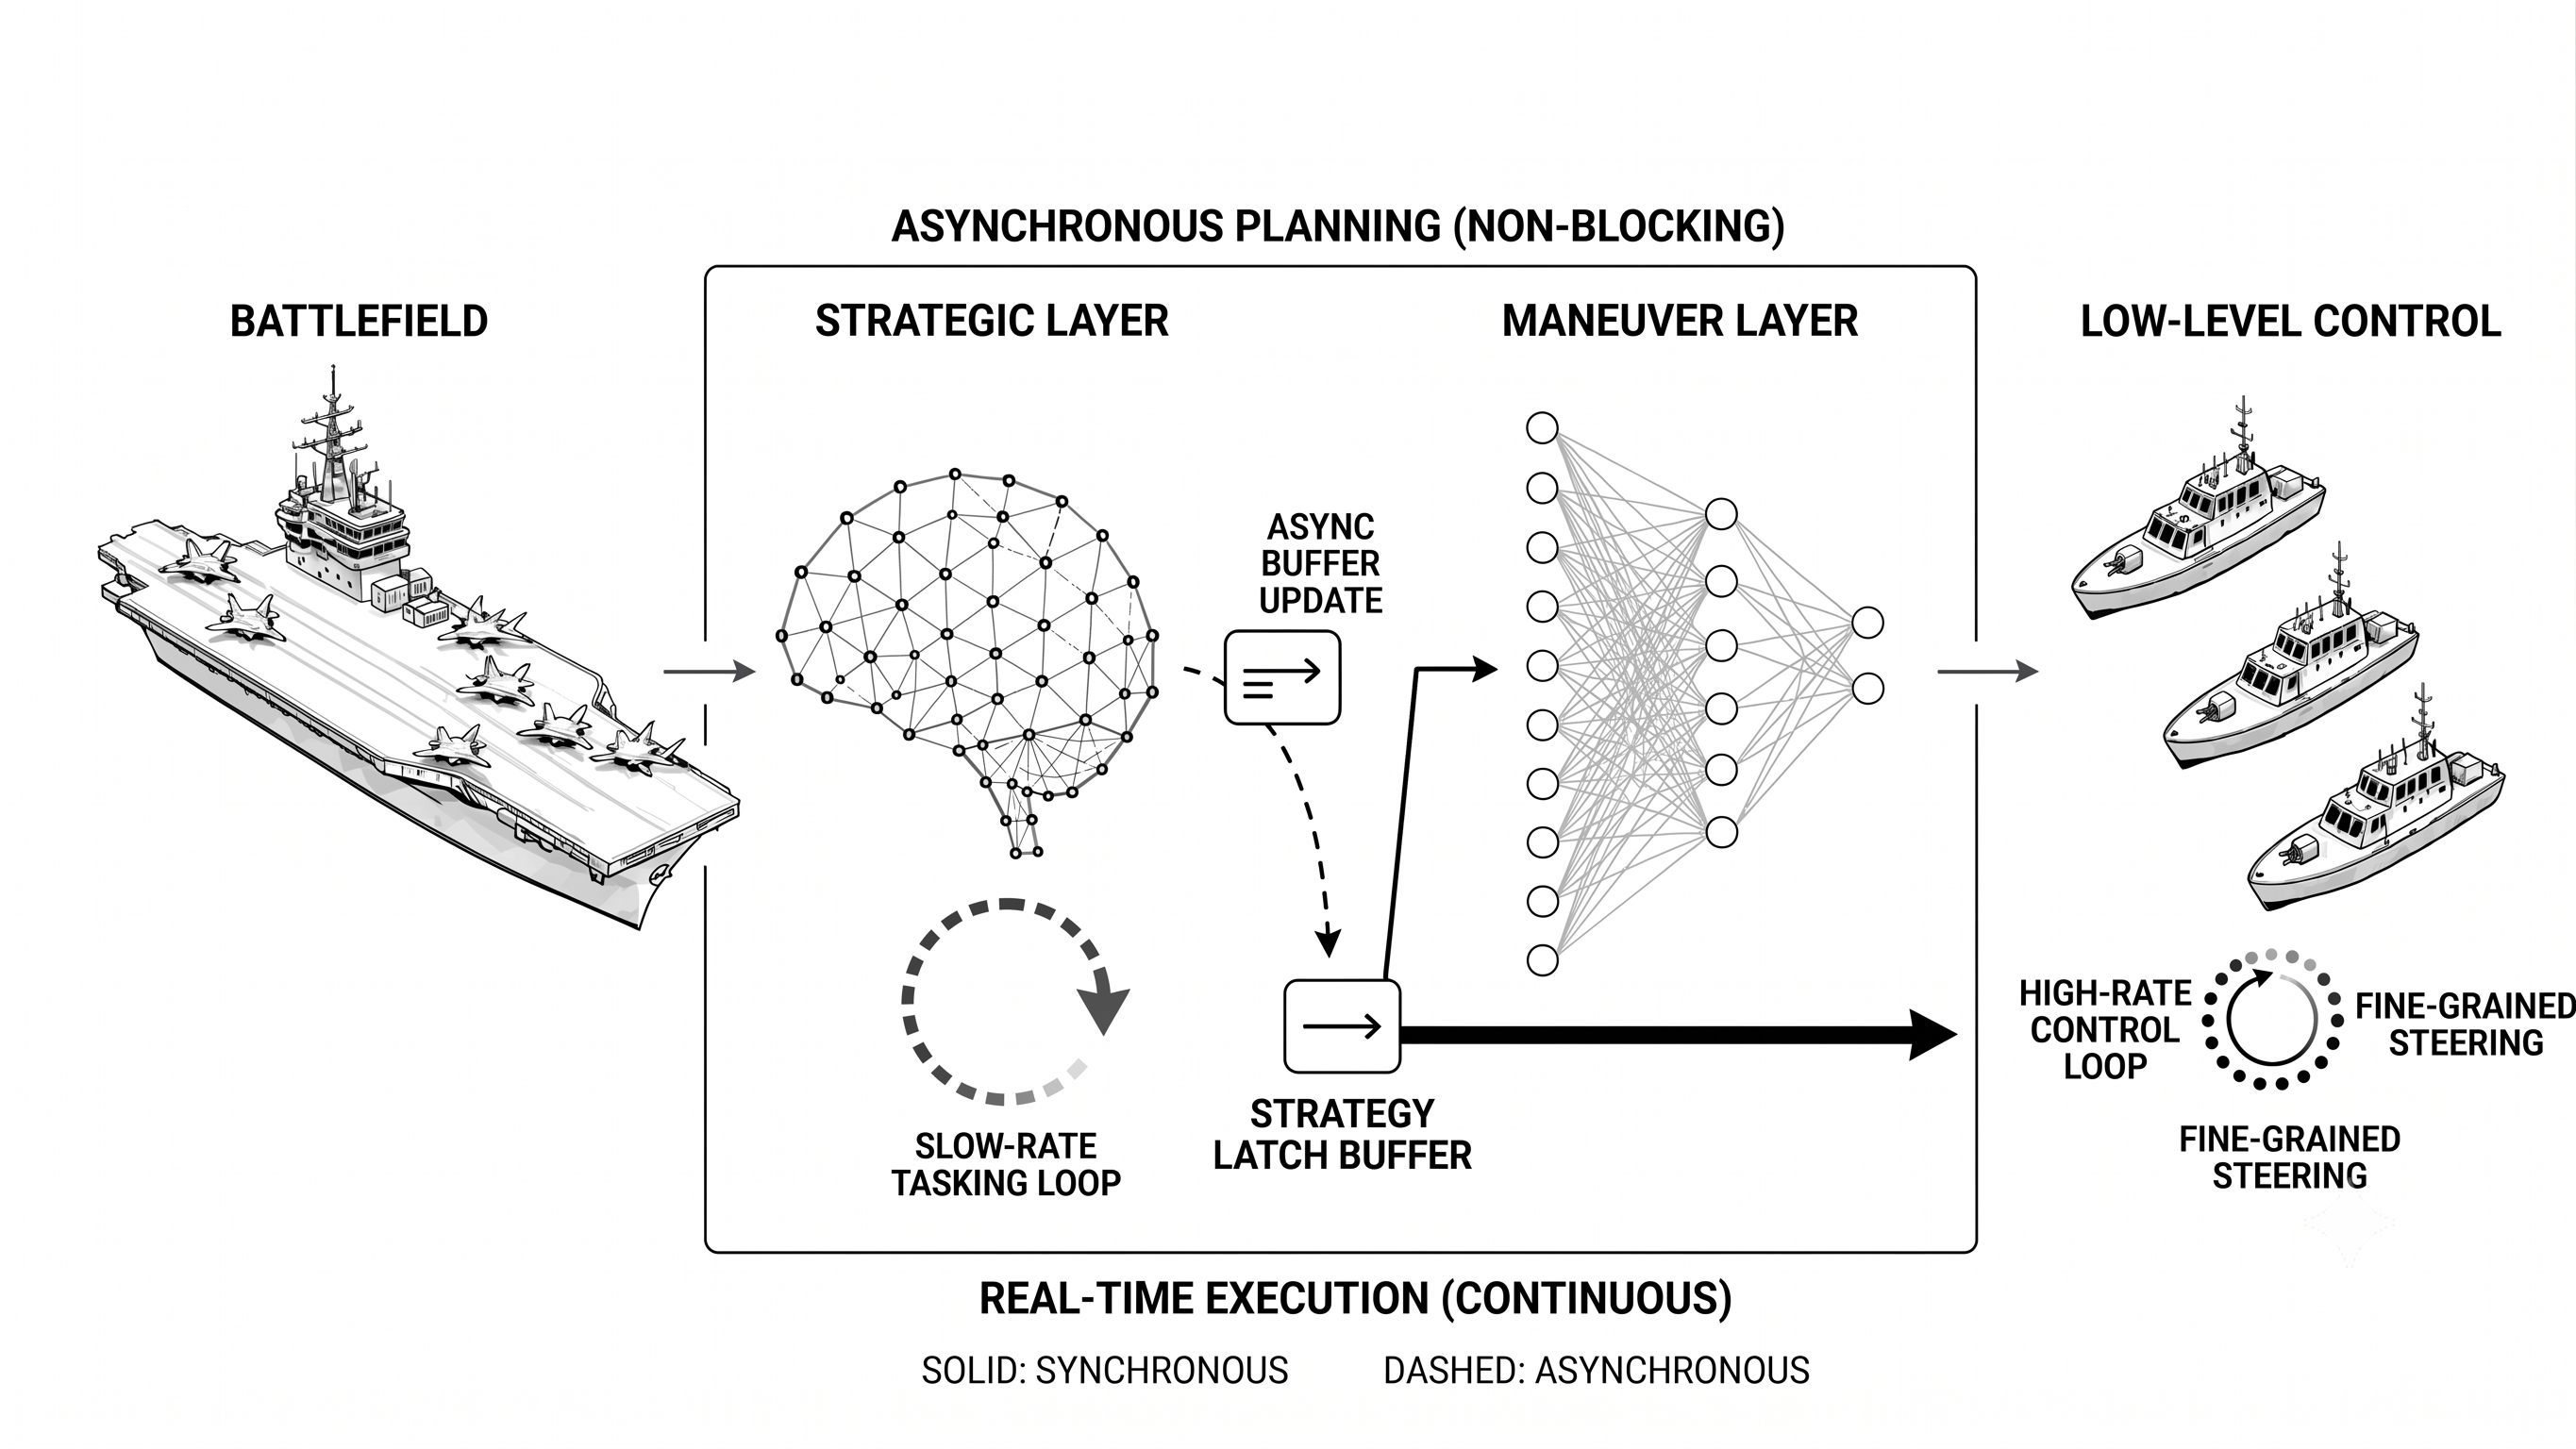
\includegraphics[width=0.72\textwidth]{fig4.png}
\caption{제안 체계의 2계층 구조}
\label{fig:architecture}
\end{figure*}

최근 분쟁에서는 폭약을 실은 값싼 무인수상정(USV) 여러 척이 여러 방향에서 동시에 고가치
함정으로 돌진하는 자폭 USV 공격이 새로운 비대칭 위협으로 떠오르고 있다. 기존 방어 수단으로는
이 공격을 막기 어렵다. 첫째, 함정이 한 번에 상대할 수 있는 요격 수단보다 자폭 USV가 많으면,
아무리 효율적으로 배정해도 표적이 남는다~\citep{ahuja2007wta}. 둘째, 전파 교란이나 기만처럼
표적을 파괴하지 않고 무력화하는 연성 대응(soft-kill)은 광섬유 같은 유선으로 조종되는 표적에는
통하지 않는다~\citep{wang2021cuas, sutea2026fiber}. 셋째, 함포나 유도탄으로 표적을 직접
파괴하는 경성 대응(hard-kill)은 값싼 표적 하나에 비싼 유도탄을 써야 해서 비용이 맞지 않는다.
표적이 한꺼번에 몰려와 대응 능력을 넘어서는 포화 상황 또한 문제이다~\citep{rumbaugh2024cost}.

본 연구는 값싼 그물로 표적을 물리적으로 붙잡는 방식을 택한다~\citep{wang2021cuas}. 그물은
표적이 무선으로 조종되든 유선으로 조종되든 똑같이 무력화한다. 다만 방어정은 자폭 USV보다
느려서 뒤쫓을 수 없다. 그래서 적이 지나갈 접근 경로에 먼저 가서 그물로 가로막는다.

이를 위해서는 두 가지를 판단해야 한다. 하나는 어느 방어정이 어느 자폭 USV를 맡을지 정하는
배정이고, 다른 하나는 그 표적을 어디에서 막을지 정하는 기동이다. 본 연구는 배정을 언어모델
지휘관에게, 기동을 강화학습으로 학습한 정책에 맡긴다. 언어모델은 답을 내는 데 오래 걸리지만,
학습된 정책은 신경망을 한 번 계산하는 것만으로도 행동을 산출해낸다. 두 판단은 걸리는 시간이
크게 다르므로, 기동이 언어모델의 응답을 기다리느라 늦어지지 않도록 느린 배정 계층만 비동기로
분리하여 기동 정책은 매 주기 지체 없이 행동하도록 구현한다(Fig.~\ref{fig:architecture}).

학습과 평가는 OpenStreetMap 해안선으로 만든 실해역 지형에서 수행한다. 기동 정책은 모선 중심
격자 지도를 영상으로 입력받아 그 지도에서 목표 격자 하나를 고르며, 갈 수 없는 격자는 후보에서
미리 제외한다. 고른 격자는 제어 명령이 아니라 경유점으로 디코딩되며, 정책은 그 지점까지 배를
모는 저수준 추종과 분리된다(\ref{sec:method}절). 배정과 기동의 기여는 각 계층을 휴리스틱과 제안
방법 중 하나로 두는 네 조합을 같은 시나리오에서 비교해 측정한다(\ref{sec:experiment}절).
